% !TEX program = XeLaTeX
\documentclass[review]{elsarticle}

\usepackage{lineno,hyperref}
\usepackage{array, pbox}
\usepackage{mathtools}
% \usepackage{colortbl}
\usepackage[table]{xcolor}
\usepackage{caption}

\definecolor{DeepRed}{HTML}{990000}
\definecolor{DarkSalmon}{HTML}{ea9999}
\definecolor{Salmon}{HTML}{f4cccc}

\definecolor{DeepPurple}{HTML}{674ea7}
\definecolor{DarkLiliac}{HTML}{b4a7d6}
\definecolor{Liliac}{HTML}{d9d2e9}

\definecolor{DeepGreen}{HTML}{6aa84f}
\definecolor{DarkLime}{HTML}{b6d7a8}
\definecolor{LightGreen}{HTML}{d9ead3}

\definecolor{DarkBlue}{HTML}{6d9eeb}
\definecolor{LightBlue}{HTML}{c9daf8}

\definecolor{Plum}{HTML}{a64d79}
\definecolor{LightPlum}{HTML}{c27ba0}
\definecolor{Mustard}{HTML}{ffd966}
\definecolor{DeepSalmon}{HTML}{e06666}

\makeatletter
\newcommand*{\@rowstyle}{}
\newcommand*{\rowstyle}[1]{% sets the style of the next row
  \gdef\@rowstyle{#1}%
  \@rowstyle\ignorespaces%
}
\newcolumntype{=}{% resets the row style
  >{\gdef\@rowstyle{}}%
}
\newcolumntype{+}{% adds the current row style to the next column
  >{\@rowstyle}%
}
\makeatother

\modulolinenumbers[5]
\journal{Journal of Information Processing and Management}

%%%%%%%%%%%%%%%%%%%%%%%
%% Elsevier bibliography styles
%%%%%%%%%%%%%%%%%%%%%%%
%% To change the style, put a % in front of the second line of the current style and
%% remove the % from the second line of the style you would like to use.
%%%%%%%%%%%%%%%%%%%%%%%

%% Numbered
%\bibliographystyle{model1-num-names}

%% Numbered without titles
%\bibliographystyle{model1a-num-names}

%% Harvard
%\bibliographystyle{model2-names.bst}\biboptions{authoryear}

%% Vancouver numbered
%\usepackage{numcompress}\bibliographystyle{model3-num-names}

%% Vancouver name/year
%\usepackage{numcompress}\bibliographystyle{model4-names}\biboptions{authoryear}

%% APA style
%\bibliographystyle{model5-names}\biboptions{authoryear}

%% AMA style
%\usepackage{numcompress}\bibliographystyle{model6-num-names}

%% `Elsevier LaTeX' style
\bibliographystyle{elsarticle-num}
%%%%%%%%%%%%%%%%%%%%%%%
\begin{document}

\begin{frontmatter}

\title{Measuring the Influence of Mere Exposure Effect of TV Commercial Adverts on Purchase Behavior based on Machine Learning Prediction Models}

\author[gidai]{Elisa Claire Alemán Carreón
\corref{mycorrespondingauthor}}
\ead{s153400@stn.nagaokaut.ac.jp}

\author[gidai]{Hirofumi Nonaka}
\ead{nonaka@kjs.nagaokaut.ac.jp}

\author[gidai]{Asahi Hentona}
\ead{s173348@stn.nagaokaut.ac.jp}

\author[gidai]{Hirochika Yamashiro}
\ead{s173358@stn.nagaokaut.ac.jp}

\address[gidai]{Nagaoka University of Technology, Nagaoka, Japan}


\cortext[mycorrespondingauthor]{
Corresponding author%: \\
% Elisa Claire Alemán Carreón \\
% Mailing Address: P.C. 940-2033, Ribbon Nagaoka B104, 1128-3 Kaminozoki-machi, Nagaoka, Niigata, Japan \\
% Cell Phone: 080-9869-4756 \\
}


\begin{abstract}
Since its introduction, television has been the main channel of investment for advertisements in order to influence customers purchase behavior. Many have attributed the mere exposure effect as the source of influence in purchase intention and purchase decision; however, most of the studies of television advertisement effects are not only outdated, but their sample size is questionable and their environments do not reflect reality. With the advent of the internet, social media and new information technologies, many recent studies focus on the effects of online advertisement, meanwhile the investment in television advertisement still has not declined. In response to this, we applied machine learning algorithms SVM and XGBoost to construct a number of prediction models based on advertisement exposure time, examining the predictability of Purchase Intention and Actual Purchase behaviors of 3000 customers across 38 different products during the span of 3 months. If we were able to predict purchase behaviors based on exposure time only, the obvious strategy for businesses would be to increase the number of adverts. On the other hand, unpredictability would put doubts in the effectiveness of the hard investment in television advertising. With our user-based predictability analysis, we found that only a fourth of the population was predictable in regards to their Purchase Intention, and that exposure to advertisements doesn't relate to Actual Purchase behaviors in any observable way. With our product-based analysis, only a few products produced predictability in Purchase intention, and none were able to influence Actual Purchase predictions. This has immense implications for the advertisement industry, since the return of investment in advertisement cannot be predicted accurately, and the effectiveness of television advertisements in increasing sales is now doubtful.


\paragraph{Highlights}
\begin{itemize}
\setlength\itemsep{-0.5em}
\item Exposure time to adverts was not found to induce predictability of purchase behavior.
\item Purchase Intention is only slightly predictable, and no link to Actual Purchase behavior was found.
\item Actual Purchase behavior was completely unpredictable, regardless of exposure to advertisement. 
\item Based on mere exposure effect only, effectiveness of television advertisement in increasing sales was not observed.
\end{itemize}

\end{abstract}

\begin{keyword}
Television Adverts\sep
Purchase Behavior\sep
SVM\sep
XGBoost\sep
Machine Learning
\end{keyword}

\end{frontmatter}

\linenumbers

\section{Introduction}
\label{intro}

It is generally thought that in order for companies to increase sales, they must somehow increase the purchase intention of their potential customers \cite{1,2}. Historically this has been approached through many channels, but since the successful introduction of the television to the general public, it has been largely attempted via television commercial advertisements, and many companies invest heavily on these efforts. However, most studies to prove the effectiveness of these advertisements have been conducted on small sample groups, usually introducing a customer to a commercial advertisement and measuring their intentions to purchase a product before and after watching the advertisement with a survey \cite[e.g.][]{3}. Studies on the predictability of purchase behavior from purchase intention data have pointed out that many of these analyses have very different results \cite{2,4,5}, presumably because of small and non-representative samples, and controlled environments that do not reflect reality. 

With the advent of Big Data and new methodologies in the field of information technology, there is a new and improved lens for advertisement research in real environments; however, its focus is mostly on similarly new advertisement online and in social media \cite{6,7,8,9}, leaving behind the study of more traditional advertisement which has not declined in use since the increase of online advertisement. In response to this lack of current research in the field of television advertisement, we propose a machine learning approach to this problem, with a large database of the television usage timelines of surveyed individuals and their answers regarding recent purchase intentions and actual purchase recalls at two points in time separated by 3 months, provided by the Nomura Research Institute, Ltd. 

Now, following the traditional train of thought of the effects of mere exposure \cite{10}, we propose collecting the accumulated number of seconds that a user has viewed a commercial advert related to a certain product and observe its effects on the users. With this data we propose training a model to predict the purchase intention and purchase recall of users based on the amount of accumulated seconds of being exposed to the advertisement for the related product in the survey. We propose to do this by unit of product, to observe the difference in marketing success from product to product, and by unit of user, to observe the rate of population that was potentially influenced by advertisements. This introduces both granularity, as we are using precise television viewing time and observing effects over time, and the potential of generalizing our prediction model to unknown new users or products after training.

\section{Research Objective}
\label{resobj}

The objective of this study is to provide an updated methodology and a larger scale database to measure the mere exposure effect and perceptual fluency effect of television adverts on purchasing behavior. For a long time, psychology based studies have been widely performed on small groups of people in very controlled environments that do not reflect customers in real life accurately, and they have been traditionally thought effective without criticism. We aim to measure the predictability in purchase behavior based on the time spent exposed to adverts of specific products in a real environment during the duration of 3 months, and provide a clearer answer to whether the heavy investment into TV advertising is actually having an effect on customers to purchase more. In the case that the predictability is high enough, this methodology could be used as a measure for future sales. On the other hand, a low predictability would create doubts on whether the mere exposure to advertisements on television is being effective.

\section{Related Work}
\label{related}

In previous research, there have been attempts to analyze the effects of adverts via mere exposure \cite{11}, and many studies have replicated the original experiment by Zajonc unrelated to adverts in the field of psychology \cite{12,13}. Now, in addition to the focus on the mere exposure effect, there have been attempts to measure the effects of advertisements on brand recognition and perception fluency \cite{14}, as well as its effects on the perception of the product \cite{15}. Fluency is defined as the level of ease or difficulty with which external information is processed \cite{16}. Previously it has been proven that it can produce bias, and it has been shown to affect the judgement of truth \cite{17}. For a long time, the perceptual fluency model has stated that repeated exposure leads to a more readily accessibility of the target brand in memory, which in turn must have an effect on the ability to recognize a brand in the future \cite[e.g.][]{18}. Most of the older research had arrived to a consensus that there is a positive influence \cite{19, 20}. More recent research, however, explores further whether these effects in memory are strictly related to positive emotional judgment on the brands or if they can also imply negative judgements based on the main objective of a product. \cite{21}. 

Research of the direct effects of television advertisement has also been attempted. One study focuses on child obesity by using weight measurements \cite{22}. An even more direct approach has been made in another study which has used brain imaging in order to explore the short-term and long-term memory effects of TV commercials \cite{23}. It should be noted that, as is to be expected in a brain imaging experiment, the participants observed the advert directly and more consciously than in mere exposure experiments. 

Now, two of the main issues with these studies and others in television advertisement effects are that, not only is the size of the samples in these experiments questionably small, but the environment is limited in that it becomes extremely controlled, to the point where it doesn't reflect the reality of customers watching daily television and making purchases anymore, and the observations environment itself could affect the results. 

In order to solve this limitation, our research is based in data science analysis methodology, such as machine learning algorithms trained from large samples of data. Current big data analysis on advertising is mostly focused on online advertisements \cite{9, 24}, where, with the advance of current technology, a user is exposed to adverts placed near to the the content they are currently consuming which are specifically targeting their interests \cite{25,26}, catching their attention (which is no longer mere exposure, but direct interaction), or a user is incentivized to watch an advertisement by blocking completely the content they were consuming until the advertisement is finished playing on screen. Most of the research in this area is focused on new ways to create online advertisements in social media \cite{27} and suggestions or recommendations targeted to a user's interests \cite[e.g.][]{28,29,30,31} reducing the need of mere exposure advertisement while online. In addition to this, some studies have focused on testing the effects of online advertisement on customers \cite{32,33,34}.

While these new technologies made possible the analysis of online advertisement and social media, the focus has shifted and there is no research using these technologies to test the effectiveness of the mere exposure effect based advertisements which are still in use in other traditional means, such as billboards, or as we analyze in our study, television advertisement. Our study is unique in that, using data from television advertisement and not online ads, we apply data science methodology to explore with a larger sample and a real life environment if there is an effect caused by mere exposure advertisement, and to what extent this effect happens. 

\section{Methodology}
\label{method}

As explained above, our approach is to train machine learning models based on the number of seconds of advertisement exposure, to predict the effect on the customers purchase decisions. A high predictability would be useful for measuring and predicting sales in any industry. On the other hand, a low predictability would create doubts that the current advertisement based on mere exposure is effective.

Our proposed method is explained in detail in the following sections.

\subsection{Survey Data Analysis}
\label{survey_data_analysis}

\subsubsection{Purchase Intention and Actual Purchase}
\label{pi_and_ap}

From the survey data provided by Nomura Research Institute Ltd., we can examine 3000 customer samples, of which we can extract the Purchase Intention and Actual Purchase answers at two points in time, one in January 2017, and another in March 2017, for 200 different products. Each time, the surveys inquire the customer if they have recently had an intention or desire to purchase a certain product (regardless of action on this desire), which corresponds to Purchase Intention; likewise, it inquires if they have recently had purchased a product, corresponding to the Actual Purchase element. We will inspect the effect of adverts on these two elements of a customer's purchase decisions and observe their change with time on the span of three months.

\subsubsection{Data Categorization}
\label{data_cat}

In order to explore the different effects commercial adverts may have on the purchase decisions of customers based on their answers from two different points in time, we have labeled each user in regard to each product with 6 categories (from 0 to 5), describing several patterns of behavior. For example, let's examine customers who answered they had purchased a product in January and then not in March, corresponding to category 0, in comparison to customers who purchased the product in March, corresponding to category 4: It is possible that, had category 0 customers were exposed to adverts in greater quantity than other users who still purchased the product and weren't exposed to as many adverts on the span of 3 months, this could mean that the advert was at least not effective, or in a worse scenario, off-putting. On the other hand, if the amount of advert exposure was minimal with category 0 customers and at the same time, customers in category 4 who actually recall having purchased the product in the March survey had been exposed to a large amount of adverts, it would prove to be an effective commercial advert campaign.

Although our approach for analysis is different, the above is a simple example of the importance of this distinction between behavior categories. The six categories for each element are explained in detail in Table \ref{tab:categories_ap} and Table \ref{tab:categories_pi}.

\begin{table} \centering
\caption{Category definition for Actual Purchase element}\label{tab:categories_ap}
\rowcolors{2}{DarkSalmon}{Salmon}
\begin{tabular}{|=c|>{\centering\arraybackslash}+m{13em}|>{\centering\arraybackslash}+m{13em}|}\arrayrulecolor{white}\hline
\rowcolor{DeepRed}
\rowstyle{\color{white}\bfseries}
Category & January Actual Purchase & March Actual Purchase \\ \hline
0 & Yes & No \\ \hline
1 & No & No \\ \hline
2 & No & Yes \\ \hline
3 & Yes & Yes \\ \hline
4 & Not Considered & Yes \\ \hline
5 & Not Considered & No \\ \hline
\end{tabular}
\end{table}

\smallskip

\begin{table} \centering
\caption{Category definition for Purchase Intention element}\label{tab:categories_pi}
\rowcolors{2}{DarkLiliac}{Liliac}
\begin{tabular}{|=c|>{\centering\arraybackslash}+m{13em}|>{\centering\arraybackslash}+m{13em}|}\arrayrulecolor{white}\hline
\rowcolor{DeepPurple}
\rowstyle{\color{white}\bfseries}
Category & January Purchase Intention & March Purchase Intention \\ \hline
0 & Yes & No \\ \hline
1 & No & No \\ \hline
2 & No & Yes \\ \hline
3 & Yes & Yes \\ \hline
4 & Not Considered & Yes \\ \hline
5 & Not Considered & No \\ \hline
\end{tabular}
\end{table}

\subsection{Advert Viewing Time Calculation}
\label{advert_viewtime_calc}

Now, on the other side of our analysis, observing the relation between the previously explained data and the effectiveness of commercial adverts on television, we extract the viewing time for adverts of each product for each customer from the television viewing data provided by Nomura Research Institute Ltd. Now the data provided tells us if a user had the television on at the moment of a certain show. Using the information provided of which commercial advert was shown during which television show and how long they lasted, we extracted the number of accumulated seconds a user had the television on for the adverts of each product, and organized them into different weekdays and time slots. We did this to further analyze whether the time period regularly described as "Primetime" had any different influence than other time slots. The final data for each user and product included the elements described in Table \ref{tab:viewtimes}. We created different datasets so that the viewing time of one element never repeated in a later one. Because of this, the total viewing time was analyzed on its own.

\begin{table} \centering
\caption{Viewing time analysis elements}\label{tab:viewtimes}
\begin{tabular}{|>{\columncolor{DarkLime}\bfseries}l|>{\columncolor{LightGreen}}m{25em}|} \arrayrulecolor{white}\hline
\rowcolor{DeepGreen}
\multicolumn{1}{|c|}{\color{white}\textbf{Viewing Time}} & \multicolumn{1}{c|}{\color{white}\textbf{Notes}} \\ \hline
Monday & Monday Primetime only, Non Primetime only, and Total. \\ \hline
Tuesday & Tuesday Primetime only, Non Primetime only, and Total. \\ \hline
Wednesday & Wednesday Primetime only, Non Primetime only, and Total. \\ \hline
Thursday & Thursday Primetime only, Non Primetime only, and Total. \\ \hline
Friday & Friday Primetime only, Non Primetime only, and Total. \\ \hline
Saturday & Saturday Primetime only, Non Primetime only, and Total. \\ \hline
Sunday & Sunday Primetime only, Non Primetime only, and Total. \\ \hline
Weekday & Five Weekdays Primetime only, Non Primetime only, and Total. \\ \hline
Weekend & Saturday and Sunday Weekend. Primetime only, Non Primetime only, and Total. \\ \hline
Holidays & Weekdays that are also Holidays. Primetime only, Non Primetime only, and Total. \\ \hline
Rest Day & Weekday Holidays and Weekends together. Primetime only, Non Primetime only, and Total. \\ \hline
Primetime & All days included, total Primetime advert viewing. \\ \hline
Non Primetime & All days included, total Non Primetime advert viewing.  \\ \hline
Total & Total amount of accumulated seconds viewed of adverts. \\ \hline
\end{tabular}
\end{table}

\subsection{Support Vector Machine}
\label{svm}

Support Vector Machines (later abbreviated SVM) are supervised machine learning models used in regression and classification problems \cite{35}. Supervised learning meaning that the model trains on previously labeled data, and establishes a way to match the labels as accurately as possible for new unlabeled data to be analyzed. In a binary classification problem, also called a Support Vector Classifier (SVC), previously established binary labels are matched with a p-dimensional vector of input data. Each column or dimension in the vector expresses a feature in the input data, and each row of the vector is a different data point. After each data point is matched with a label, an SVM uses an algorithm to determine a (p-1)-dimensional hyperplane that separates the p-dimensional space in a way that minimizes error in classification, by maximizing the distance between the hyperplane and the nearest point in either classification. A two-dimensional example is shown in Figure \ref{fig:svm}.

% Insert figure 1
\begin{figure}
\centering
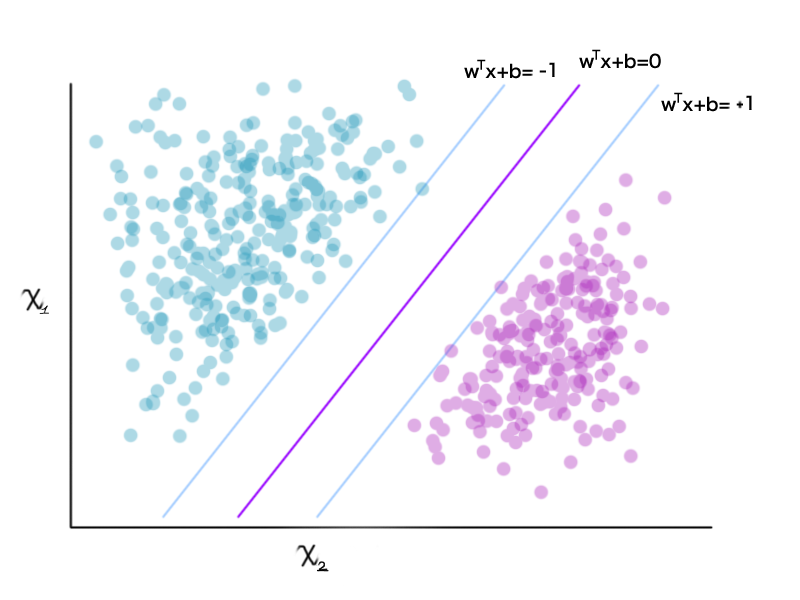
\includegraphics[width=20em]{figures/SVM_2d_example.png}
\caption{Two dimensional example of an SVM classification problem}
\label{fig:svm}
\end{figure}

In our study we used the linear kernel for our SVC, defined by the formula (\ref{eq:1}) below, where \(x\) is the input vector, \(w\) is the weight vector, and \(b\) is the bias vector. The dimensions of these vectors are such that \(f(x)\) and \(b\) are the size of the sample size, and \(w\) is the size of the amount of features. The sign of the value of \(f(x)\) determines which classification label \(y\) is applied, as shown in the formulas (\ref{eq:2}) and (\ref{eq:3}). 

\begin{equation}\label{eq:1}
f(x) = w^\top x + b
\end{equation}

\begin{equation}\label{eq:2}
f(x)\geq 0 \rightarrow y= +1 
\end{equation}

\begin{equation}\label{eq:3}
f(x)\leq 0 \rightarrow y= -1 
\end{equation}

The algorithm consists of, starting with a weight and bias vector comprised of zeroes, a randomly placed hyperplane is drawn. Each data point is tested for correct classification, and if the classification fails, the value of \(w\) is changed by a value of \(\alpha\) as follows (\ref{eq:4}). Finally the distance to the nearest points, the support vectors, in either classification, called the margin, is calculated.

\begin{equation}\label{eq:4}
w \leftarrow w + \alpha  sign(f(x_{i}))x_{i}
\end{equation}

This process is repeated so that the margin is maximized and the number of erroneous classifications are minimized. 

Now, in order to measure the effectiveness of the training process and data, we perform what is called a K-fold cross validation. This means that after randomly shuffling and splitting our training data in k equal parts, k-1 of those parts are used for training, while the remaining one part is used in validation. Using the trained SVM, a prediction is made, and it is decided if such a prediction is correct or not, and counted and grouped as a True Positive, True Negative, False Positive or False Negative prediction. This is explained in Table \ref{tab:preds}.

\begin{table} \centering
\caption{Prediction outcomes}\label{tab:preds}
\begin{tabular}{|>{\centering\arraybackslash}m{7em}|>{\centering\arraybackslash}m{7em}|>{\centering\arraybackslash}m{7em}|} \arrayrulecolor{white}\hline %\cline{2-3}
\multicolumn{1}{c|}{} & \cellcolor{Mustard}\textbf{Prediction is Correct} & \cellcolor{LightPlum}\textbf{Prediction is Incorrect} \\ \hline
\cellcolor{DarkBlue}\textbf{Prediction is Positive} & \cellcolor{DeepGreen}True Positive & \cellcolor{DeepPurple}False Positive \\ \hline
\cellcolor{DeepSalmon}\textbf{Prediction is Negative} & \cellcolor{orange}True Negative & \cellcolor{Plum}False Negative \\ \hline
\end{tabular}
\end{table}

Measures of accuracy are determined from these prediction outcomes. This process is then repeated \(k\) times and the measures taken are averaged. In this study we used the \(F_{1}\) score, which measure is a harmonic mean between precision and recall. Precision, described in formula (\ref{eq:5}), lets us observe the rate of correct positive predictions from all the positive predictions, while Recall, detailed in formula (\ref{eq:6}), observes the rate of correct positive predictions from the total of actual positive data. The \(F_{1}\) score in formula (\ref{eq:7}) then can only be high when both of these measures are high simultaneously, and will lower substantially if they are not consistent. We use this score as it allows us to avoid overlooking data while maintaining accurate predictions.

\begin{equation}\label{eq:5}
Precision = \frac{True Positives}{True Positives + False Positives}
\end{equation}

\begin{equation}\label{eq:6}
Recall = \frac{True Positives}{True Positives + False Negatives}
\end{equation}

\begin{equation}\label{eq:7}
F_{1} = 2  \frac{Precision * Recall}{Precision + Recall}
\end{equation}

\subsection{XGBoost}
\label{xgboost}

Originally started as a research project by Tianqi Chen \cite{36}, XGBoost is an improved and optimized application of a Gradient Boosting Machine, or GBM, also called gradient tree boosting, or gradient boosted regression tree. A Gradient Boosted Regression Tree (GBRT) works by building an ensemble model from several weak learning machines which are just above random guessing in accuracy, in this case using Decision Trees. The misclassified results from these weak predictions are then weighted and added to a final strong learning machine. This process iteratively optimizes the misclassification cost in a functional gradient descent so that the final learning machine focuses on important factors from the training data for a stronger prediction model. 

\section{Experiments}
\label{experiments}

\subsection{Prediction Models}
\label{pred_models}

Based on the input vector that is used, we have proposed investigating the two different configurations possible for our prediction models, as explained in Table \ref{tab:modelbases}.

\begin{table} \centering
\caption{Prediction Model Bases}\label{tab:modelbases}
\begin{tabular}{|>{\raggedright\arraybackslash}=m{10em}|+m{22em}|} \arrayrulecolor{white}\hline
\rowcolor{Plum}\rowstyle{\color{white}\bfseries}
Prediction Model Base & Description \\ \hline
\rowcolor{LightBlue}
\pbox{10em}{\cellcolor{DarkBlue}\textbf{Product Based} \\ \textbf{Prediction Models}} & For each product from 200 available in the survey, data from 3000 users was collected and paired with their labels. \\ \hline
\rowcolor{LightGreen}
\pbox{10em}{\cellcolor{DarkLime}\textbf{User Based} \\ \textbf{Prediction Models}} & For each user from 3000 available, data corresponding to all 200 products available in the survey was collected and paired with their labels. \\ \hline
\end{tabular}
\end{table}

After extracting the commercial advert viewing data using these parameters from the 3000 users that answered the survey, which includes purchase behavior questions from 200 products at two different points in time, only 38 products from those in the survey were linked to commercial adverts that were actually viewed by those same users. Thusly, we performed our experiments using the viewing data of 3000 users for these 38 products in the configurations explained before in Table \ref{tab:modelbases}.

\subsection{Prediction Model Targets}
\label{pred_model_targets}

Using the previously explained bases, we performed analysis for both Actual Purchase and Purchase Intention, and each variation in change explained before as categories in section \ref{data_cat} of this paper. With this categorization, we can observe the difference in relation between the number of seconds of advert viewing and a change in Purchase Behavior between January 2017 and March 2017. In total we performed experiments with 24 different prediction models. This can be visualized in Table \ref{tab:experiment_models}.

\begin{table} \centering
\caption{Prediction Model experiments performed}\label{tab:experiment_models}
\begin{tabular}{|=>{\centering}+m{10em}|+c|+>{\centering\arraybackslash}+m{10em}|}\arrayrulecolor{white}\hline
\rowcolor{Plum}
\rowstyle{\color{white}\bfseries}
Prediction Model & Prediction Targets & Number of Categories \\ \hline
\rowcolor{DarkSalmon}
\rowstyle{\color{black}\normalfont}
\cellcolor{LightBlue}{Product Based CM View Time} & Actual Purchase & 6 \\ \hline
\rowcolor{DarkLiliac}
\cellcolor{LightBlue}{Product Based CM View Time} & Purchase Intention & 6 \\ \hline
\rowcolor{DarkSalmon}
\cellcolor{LightGreen}{User Based CM View Time} & Actual Purchase & 6 \\ \hline
\rowcolor{DarkLiliac}
\cellcolor{LightGreen}{User Based CM View Time} & Purchase Intention & 6 \\ \hline
\end{tabular}
\end{table}

\subsection{Machine Learning Algorithms}
\label{mlalgorithms}

Using the Prediction models explained in section \ref{pred_model_targets} of this paper, we performed the machine learning experiments with both SVM and XGboost algorithms and then compared results from both groupings. 

\section{Results}
\label{results}

We investigated the relation between viewing data and 6 different purchase behavior categories depending on their change throughout two different points in time. However, the two categories which we will focus on this paper are category 2 and 4, since they represent the customer base that either changed from not purchasing to purchasing, or also customers who continued their purchases. This would let us observe if there is any positive relation between the time spent viewing commercial adverts and the purchase decision, granting us insight to the effectiveness of the advert in its desired purpose. We present the results of our analysis in the following sections. The detailed results presented first are all from the experiments performed using the SVM algorithm. We then present the differences in results for SVM and XGBoost experiments in a later section. 

\subsection{Product Based Models Results}
\label{prod_base_results}

\subsubsection{Product Based CM View Time \textperiodcentered  Actual Purchase Category 2}
\label{prod_ap_2}

For all 38 products, we collected the data of actual purchase behavior from 3000 customers, labeling those who changed their behavior from not having purchased in January 2017 to having made a purchase in March 2017 as the positive classification, and any customer other than those as the negative classification for our SVM training data.

The results of the \(F_{1}\) score for the prediction models for each of the 38 products resulted in 0. This means that any predictions were failed and that the SVM could not find a separating (p-1)-dimensional hyperplane for the viewing data. In other words, people who changed their purchasing behavior from January to March, and people who did otherwise, were exposed to similar amounts of advert time, or that viewing time was spread indiscriminately for all users regardless of purchase decision for any of the products that we investigated separately. 

\subsubsection{Product Based CM View Time \textperiodcentered  Actual Purchase Category 4}
\label{prod_ap_4}

Now, the results for the product based model labeling positively those who regardless of change, had actually purchased the product by March 2017; and labeling negatively any customers who did not purchase the product by March are presented in this section.

The \(F_{1}\) scores for all but one of the 38 prediction models in this experiment were 0. The remaining product was the japanese bottled tea "IEMON”, with an \(F_{1}\) score of 0.018. Now, for a score to describe a relatively accurate prediction model, it must be at least above 0.5. This means that even though this particular product had a score slightly above 0, there is no particular relation found by the SVM that could determine the purchase behavior of customers based on the time spent viewing adverts for the related product.

\subsubsection{Product Based CM View Time \textperiodcentered  Purchase Intention Category 2}
\label{prod_pi_2}

Similar to our results for Actual Purchase behavior, the experiment labeling positively customers whose Purchase Intention changed from not having any intention at the first point in time to having a purchase intention at the latter, and labeling negatively those who did otherwise resulted in an \(F_{1}\) score of 0 for all 38 products. This means that for any of the 38 products, advert viewing time did not have any relation to their purchase intentions changing or not in the vector space.

\subsubsection{Product Based CM View Time \textperiodcentered  Purchase Intention Category 4}
\label{prod_pi_4}

The results for Purchase Intention behavior, labeling positively customers whose Purchase Intention was positive at the latest point in time in the survey, regardless of their behavior before that point; and labeling negatively those who did otherwise, resulted in an \(F_{1}\) score greater than 0.5 for 8 of the 38 products available in our viewing data. These prediction accuracy results are presented in Table \ref{tab:results_product_pi_4}. There were other 3 products which had an \(F_{1}\) score between 0 and 0.5, not listed, and the remaining 27 products had an F1 score of 0. 

\begin{table} \centering
\caption{\(F_{1} > 0.5\) for Product Based CM View Time \textperiodcentered  Purchase Intention Category 4}\label{tab:results_product_pi_4}
\rowcolors{2}{Liliac}{Liliac}
\begin{tabular}{|l|c|} \arrayrulecolor{white}\hline
\rowcolor{DarkLiliac}
\multicolumn{1}{|c|}{\textbf{Product}} & \boldmath{\(F_{1}\)} \\ \arrayrulecolor{white}\hline
KitKat & 0.863 \\ \hline
IEMON & 0.799 \\ \hline
Ghana & 0.777 \\ \hline
Lunch Pack & 0.773 \\ \hline
Dars & 0.757 \\ \hline
Mitsuya Cider & 0.737 \\ \hline
Namacha & 0.733 \\ \hline
Jurokucha & 0.709 \\ \hline
\end{tabular}
\end{table}

\subsection{User Based Models Results}
\label{user_base_results}

This section shows the results from the user based experiments. These experiments calculate the number of specific users that are predictable in their Actual Purchase and Purchase Intention behaviors based on their advert viewing time.

\subsubsection{User Based CM View Time \textperiodcentered  Actual Purchase Category 2}
\label{user_ap_2}

This section presents the results for the Actual Purchase behavior prediction of Category 2 users (those who didn't purchase in the first survey and changed their behavior in the second survey 3 months later). Only 30 of 3000 users had an \(F_{1}\) score greater than 0.5, meaning they were fairly predictable in their behavior based on their advert viewing time. The remaining 99\% was completely unpredictable. This result is shown in Figure \ref{fig:2}.

% Insert figure 2
\begin{figure}
\centering
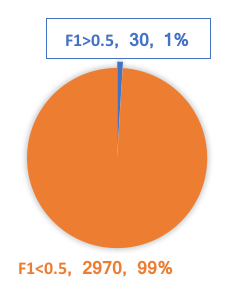
\includegraphics[width=12em]{figures/fig2.png}
\caption{Prediction results for User Based CM View Time \textperiodcentered  Actual Purchase Category 2}
\label{fig:2}
\end{figure}


\subsubsection{User Based CM View Time \textperiodcentered  Actual Purchase Category 4}
\label{user_ap_4}

The results for the user based model in Actual Purchase Category 4, however, presents a larger amount of users, with 253 of 3000 users having been predictable, obtaining an \(F_{1}\) score greater than 0.5. It is easier to predict a single purchasing behavior in their last survey, based on their viewing time from the previous 3 months, than to predict a specific change in behavior like the last experiment. However, there is still a 92\% of users whose behavior was unpredictable with only advertisement viewing time considered. This result is shown in Figure \ref{fig:3}. 

% Insert figure 3
\begin{figure}
\centering
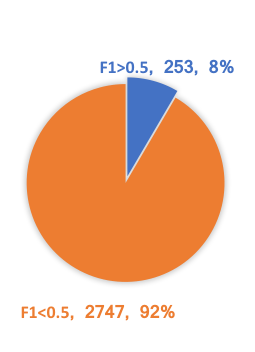
\includegraphics[width=12em]{figures/fig3.png}
\caption{Prediction results for User Based CM View Time \textperiodcentered  Actual Purchase Category 4}
\label{fig:3}
\end{figure}

\subsubsection{User Based CM View Time \textperiodcentered  Purchase Intention Category 2}
\label{user_pi_2}

Similarly to the experiment for Actual Purchase behavior, the results for Purchase Intention prediction for Category 2 users, who changed their behavior from not purchasing to purchasing between surveys, was extremely low. Only 40 of the 3000 users had a prediction score greater than 0.5. This result is shown in Figure \ref{fig:4}. 

% Insert figure 4
\begin{figure}
\centering
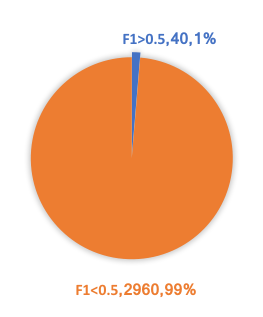
\includegraphics[width=12em]{figures/fig4.png}
\caption{Prediction results for User Based CM View Time \textperiodcentered  Purchase Intention Category 2}
\label{fig:4}
\end{figure}

\subsubsection{User Based CM View Time \textperiodcentered  Purchase Intention Category 4}
\label{user_pi_4}

In contrast to all previous results, the user based prediction model for Purchase Intention in the last survey was more successful. 753 of 3000 users, roughly 25\% of users were predictable based on their advert viewing time regarding their Purchase Intention behavior. This result is shown in Figure \ref{fig:5}.

% Insert figure 5
\begin{figure}
\centering
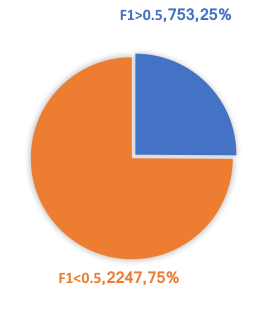
\includegraphics[width=12em]{figures/fig5.png}
\caption{Prediction Results for User Based CM View Time \textperiodcentered  Purchase Intention Category 4}
\label{fig:5}
\end{figure}

\subsection{XGBoost Comparison to SVM}
\label{svmxgboost}

As the results shown above are all from the experiments done with SVM machine learning algorithms, we show a comparison of the experiments done with XGboost in Table \ref{tab:svmxgboost_product} and Table \ref{tab:svmxgboos_user}, for product based models and user based models respectively. 

\begin{table} \centering
\captionsetup{justification=centering}
\caption{SVM and XGBoost percentage of elements with \(F_{1} > 0.5\) 
comparison for product based models}\label{tab:svmxgboost_product}
\rowcolors{2}{LightBlue}{LightBlue}
\begin{tabular}{|=c|+c|+c|} \arrayrulecolor{white}\hline
\rowcolor{DarkBlue}
\rowstyle{\bfseries}
Product Based Model & SVM & XGBoost \\ \hline
Actual Purchase Category 2 & 0 & 0 \\ \hline
Actual Purchase Category 4 & 0.08 & 0 \\ \hline
Purchase Intention Category 2 & 0 & 0 \\ \hline
Purchase Intention Category 4 & 0.21 & 0.21 \\ \hline
\end{tabular}
\end{table}

\begin{table} \centering
\captionsetup{justification=centering}
\caption{SVM and XGBoost percentage of elements with \(F_{1}>0.5\) comparison for user based models}\label{tab:svmxgboos_user}
\rowcolors{2}{LightGreen}{LightGreen}
\begin{tabular}{|=c|+c|+c|} \arrayrulecolor{white}\hline
\rowcolor{DarkLime}
\rowstyle{\bfseries}
User Based Model & SVM & XGBoost \\ \hline
Actual Purchase Category 2 & 0.01 & 0 \\ \hline
Actual Purchase Category 4 & 0.08 & 0.06 \\ \hline
Purchase Intention Category 2 & 0.01 & 0 \\ \hline
Purchase Intention Category 4 & 0.25 & 0.24 \\ \hline
\end{tabular}
\end{table}

The results for SVM prediction models held a slightly higher percentage of predictable elements, but overall they both show similar results. 

\section{Discussion}
\label{discussion}

\subsection{Influence of TV adverts on Actual Purchase and Purchase Intention}
\label{disc_ap_pi}

In this paper, we have obtained results on the predictability of Actual Purchase and Purchase Intention customer behaviors based on the time spent exposed to TV adverts. These results would not only be useful in predicting the purchasing behavior of customers, but it would be useful as a direct measure of the effectiveness of mere exposure to advertisements. However, these results are low enough that it can be said TV adverts are not a main factor in predicting whether a customer will change their purchasing behavior. While the research based on the mere exposure effect would suggest otherwise, customers are observed to decide on their purchase without much predictability. It could be said that while there is influence in the customer's knowledge of the brand, the amount of time exposed to TV adverts seems to have an indirect influence on purchasing behavior at most, if not none at all.

Other studies, using a controlled environment, have linked mere exposure with bias in consumer choice \cite{37}. However, there is a possible explanation for these discrepancies in results. While controlled experiments show the TV adverts to their sample audience directly in most cases, in an uncontrolled environment of a customer's home, the customer is left free to ignore the advert and do something unrelated in the meanwhile \cite{38}. In the United Kingdom, there is a widely documented phenomenon involving TV advert timing and a surge in electricity caused by the use of electric kettles for preparing tea. This phenomenon is commonly called TV pickup, and has been documented for long \cite{39,40}. Similar to these cases, if the customers whose data were actively ignoring the adverts, the sample for training the prediction models would contain noise, altering the results. It stands to reason that without the influence of this active aversion would have on our learning model, it might correctly predict purchasing behavior as expected. However, this is more of a problem with the current TV advertisement model than with the methodology of this study. We will discuss this further in section \ref{disc_advert} of this paper.


\subsection{Influence of TV adverts based on Primetime}
\label{disc_prime}

In our prediction model experiments, we used data from advertisement exposure during different time periods, days of the week and weekends. While we did this in order to observe differences in predictability for different time schedules available to different kinds of customers, especially during primetime television hours, we arrived to similarly low results for all time categories. We did not observe any difference in predictability based on Primetime television watching compared to other time periods, as well as differences in weekdays and weekends. This could be interpreted as there being little influence in time periods and changes in purchasing behavior. However, as we stated in section \ref{disc_ap_pi}, the common problem with advertisements being actively ignored by customers has existed for long. Taking this problem into consideration, our results imply that the problem is constant over all the time periods, and that there is not a particular time slot that results in customers being more attentive to adverts.

\subsection{Implications for the TV advert industry}
\label{disc_advert}

Based on the low results of predictability of purchase behavior by advert exposure, it can be observed that TV adverts have a low probability of achieving their main purpose: to increase sales. As was stated in section \ref{disc_ap_pi} of this paper, there could be a large influence on this study's results from customers actively ignoring the adverts although they are being broadcast to their TVs. It is left to further discussion and research if adverts actually have the intended effect on customers when watched properly, or if this effect is not achieved anyway. In \cite{14} it is proposed that while the mere exposure of banner advertisement increases perceptual fluency, it doesn't have an effect on actual brand recognition compared to the control groups, for example. The existence or absence of influence by perceptual fluency on a customer's purchase decision hasn't been fully explored, but the consensus in the processing fluency model is that perceptual fluency influences brand judgement on some level, although it depends on the concept if the reception is positive or not \cite{21}. The problem with these studies and the current consensus, as has been said previously in this paper, is both that most experiments are done with relatively small sample sizes, and that there is a factor of uncertainty that comes with the physical avoidance of adverts in a customers home environment.

With these things in mind, we consider both possibilities: either customers are attentive and the adverts have the expected influence in their short and long term memories in the case of repeated exposures \cite{23}; or the customers are inattentive of the advert and there might be some level of unconscious effect of mere exposure in their perception fluency \cite{14}. We observed however in our results that the effect on Actual Purchase behavior is minimal. While it may be true and out of the reach of our data that the customers would have influence in their memory, there was no link observed between the time of advert exposure and the purchase decisions. This raises a concern for the TV advert industry. Regardless of the cause of our results, the main implication of our paper is that currently, TV adverts are shown to have little to no effect on changes in Actual Purchase behavior, and only some observable effect in Purchase Intention. While thousands of billions of japanese yen are spent on TV advertisements each year \footnote{\label{dentsu}Dentsu, inc. 2017 Advertising Expenditures in Japan. Retrieved on May 2018 from \href {http://www.dentsu.com/knowledgeanddata/ad_expenditures/pdf/expenditures_2017.pdf}{\path{http://www.dentsu.com/knowledgeanddata/ad_expenditures/pdf/expenditures_2017.pdf}}}, the effects observed in this study are negligible. Because of this, changes are necessary in the current TV advertisement model.

\section{Conclusion and Future Work}
\label{conclusion}

In this paper we analyzed the ability to predict purchasing behavior, namely Purchase Intention and Actual Purchase based on the customers' time spent exposed to television adverts using machine learning algorithms. We analyzed the data by product and by customer, determining which specific products and which specific customers provided a better prediction model. Based on our low results for any prediction of Actual Purchase, we concluded that there must be other factors that are more strongly tied to the customer's purchasing behavior. The results for Purchase Intention were relatively higher but still low enough that only a few products, mostly tea and chocolate snacks, could be predicted, and only one fourth of the customers were predictable in their purchase intention. We discussed possible influence by deliberate avoidance of advert cuts to prepare food or tea, and while some studies focus on the effect of attentive watching of adverts, other studies focus on the mere exposure effects, which would be achieved despite physical avoidance because of advert audio and simple proximity of the television. Both scenarios are in strong contrast with the results of our study, which shows little to no predictability in purchase behavior. Points left to research in future work are a deeper analysis of the predictable customers, looking for similarities or clusters within this class, as well as using different machine learning algorithms, which weren't considered because of requiring bigger datasets. 

\section{Acknowledgements}

This paper was made possible by the data provided by Nomura Research Institute, Ltd. for their yearly Marketing Analysis Contest.

Declarations of interest: none

\section*{References}

\bibliography{ipmbibfile}

% \usepackage{filecontents}
% \begin{filecontents}{\ipmbibfile.bib}
% @article{1,
% author = {Armstrong, J. and Morwitz, V. and Kumar, V.},
% journal = {International Journal Of Forecasting},
% number = {3},
% pages = {383-397},
% title = {Sales forecasts for existing consumer products and services: Do purchase intentions contribute to accuracy?},
% volume = {16},
% year = {2000},
% doi = {10.1016/s0169-2070(00)00058-3},
% }

% @article{2,
% author = {Morwitz, V. and Steckel, J. and Gupta, A.},
% journal = {International Journal Of Forecasting},
% number = {3},
% pages = {347-364},
% title = {When do purchase intentions predict sales?},
% volume = {23},
% year = {2007},
% doi = {10.1016/j.ijforecast.2007.05.015},
% }

% @article{3,
% author = {Khuong, M. and Nguyen, T.},
% journal = {Journal Of Economics, Business And Management},
% number = {9},
% pages = {851-857},
% title = {The Effects of Television Commercials on Customers Purchase Intention -- A Study of Milk Industry in Ho Chi Minh City, Vietnam},
% volume = {3},
% year = {2015},
% }

% @article{4,
% author = {Sun, B. and Morwitz, V.},
% journal = {International Journal Of Research In Marketing},
% number = {4},
% pages = {356-366},
% title = {Stated intentions and purchase behavior: A unified model},
% volume = {27},
% year = {2010},
% doi = {10.1016/j.ijresmar.2010.06.001},
% }

% @article{5,
% author = {Newberry, C. and Klemz, B. and Boshoff, C.},
% journal = {Journal Of Services Marketing},
% number = {6},
% pages = {609-620},
% title = {Managerial implications of predicting purchase behavior from purchase intentions: a retail patronage case study},
% volume = {17},
% year = {2003},
% doi = {10.1108/08876040310495636},
% }

% @article{6,
% author = {Shareef, M. and Mukerji, B. and Alryalat, M. and Wright, A. and Dwivedi, Y.},
% journal = {Journal Of Retailing And Consumer Services},
% pages = {258-268},
% title = {Advertisements on Facebook: Identifying the persuasive elements in the development of positive attitudes in consumers},
% volume = {43},
% year = {2018},
% doi = {10.1016/j.jretconser.2018.04.006},
% }

% @article{7,
% author = {Gonzalez Camacho, L. and Alves-Souza, S.},
% journal = {Information Processing \& Management},
% number = {4},
% pages = {529-544},
% title = {Social network data to alleviate cold-start in recommender system: A systematic review},
% volume = {54},
% year = {2018},
% doi = {10.1016/j.ipm.2018.03.004},
% }

% @article{8,
% author = {Ramaboa, K. and Fish, P.},
% journal = {Information Processing \& Management},
% number = {2},
% pages = {175-183},
% title = {Keyword length and matching options as indicators of search intent in sponsored search},
% volume = {54},
% year = {2018},
% doi = {10.1016/j.ipm.2017.11.003},
% }

% @article{9,
% author = {Wu, C. and Kao, S. and Wu, C. and Huang, S.},
% journal = {Information Processing \& Management},
% number = {5},
% pages = {625-642},
% title = {Location-aware service applied to mobile short message advertising: Design, development, and evaluation},
% volume = {51},
% year = {2015},
% doi = {10.1016/j.ipm.2015.06.001},
% }

% @article{10,
% author = {Zajonc, R.},
% journal = {Journal Of Personality And Social Psychology},
% number = {2 Pt.2},
% pages = {1-27},
% title = {Attitudinal effects of mere exposure},
% volume = {9},
% year = {1968},
% doi = {10.1037/h0025848},
% }

% @article{11,
% author = {Hekkert, P. and Thurgood, C. and Whitfield, T.},
% journal = {Acta Psychologica},
% number = {2},
% pages = {411-417},
% title = {The mere exposure effect for consumer products as a consequence of existing familiarity and controlled exposure},
% volume = {144},
% year = {2013},
% doi = {10.1016/j.actpsy.2013.07.015},
% }

% @article{12,
% author = {Huang, Y. and Hsieh, P.},
% journal = {Vision Research},
% pages = {56-61},
% title = {The mere exposure effect is modulated by selective attention but not visual awareness},
% volume = {91},
% year = {2013},
% doi = {10.1016/j.visres.2013.07.017},
% }

% @article{13,
% author = {Dech{\^e}ne, A. and Stahl, C. and Hansen, J. and W{"a}nke, M.},
% journal = {Journal Of Experimental Social Psychology},
% number = {5},
% pages = {1117-1122},
% title = {Mix me a list: Context moderates the truth effect and the mere-exposure effect},
% volume = {45},
% year = {2009},
% doi = {10.1016/j.jesp.2009.06.019},
% }

% @article{14,
% author = {Fang, X. and Singh, S. and Ahluwalia, R.},
% journal = {Journal Of Consumer Research},
% number = {1},
% pages = {97-103},
% title = {An Examination of Different Explanations for the Mere Exposure Effect},
% volume = {34},
% year = {2007},
% doi = {10.1086/513050},
% }

% @article{15,
% author = {Gmuer, A. and Siegrist, M. and Dohle, S.},
% journal = {Food Quality And Preference},
% pages = {12-16},
% title = {Does wine label processing fluency influence wine hedonics?},
% volume = {44},
% year = {2015},
% doi = {10.1016/j.foodqual.2015.03.007},
% }

% @article{16,
% author = {Schwarz, N.},
% journal = {Journal Of Consumer Psychology},
% number = {4},
% pages = {332-348},
% title = {Metacognitive Experiences in Consumer Judgment and Decision Making},
% volume = {14},
% year = {2004},
% doi = {10.1207/s15327663jcp1404_2},
% }

% @article{17,
% author = {Silva, R. and Garcia-Marques, T. and Reber, R.},
% journal = {Consciousness And Cognition},
% pages = {53-67},
% title = {The informative value of type of repetition: Perceptual and conceptual fluency influences on judgments of truth},
% volume = {51},
% year = {2017},
% doi = {10.1016/j.concog.2017.02.016},
% }

% @article{18,
% author = {Jacoby, L. and Dallas, M.},
% journal = {Journal Of Experimental Psychology: General},
% pages = {306-304},
% title = {On the Relationship Between Autobiographical Memory and Perceptual Learning},
% volume = {110},
% year = {1981},
% }

% @article{19,
% author = {Reber, R. and Winkielman, P. and Schwarz, N.},
% journal = {Psychological Science},
% number = {1},
% pages = {45-48},
% title = {Effects of Perceptual Fluency on Affective Judgments},
% volume = {9},
% year = {1998},
% doi = {10.1111/1467-9280.00008},
% }

% @article{20,
% author = {Seamon, J. and Williams, P. and Crowley, M. and Kim, I. and Langer, S. and Orne, P. and Wishengrad, D.},
% journal = {Journal Of Experimental Psychology: Learning, Memory And Cognition},
% number = {3},
% pages = {711-721},
% title = {The Mere Exposure Effect Is Based On Implicit Memory: Effects of Stimulus Type, Encoding Conditions, and Number of Exposures on Recognition and Affect Judgements},
% volume = {21},
% year = {1995},
% }

% @article{21,
% author = {Lee, A. and Labroo, A.},
% journal = {Journal Of Marketing Research},
% number = {2},
% pages = {151-165},
% title = {The Effect of Conceptual and Perceptual Fluency on Brand Evaluation},
% volume = {41},
% year = {2004},
% doi = {10.1509/jmkr.41.2.151.28665},
% }

% @article{22,
% author = {Boyland, E. and Halford, J.},
% journal = {Appetite},
% pages = {236-241},
% title = {Television advertising and branding: Effects on eating behaviour and food preferences in children},
% volume = {62},
% year = {2013},
% doi = {10.1016/j.appet.2012.01.032},
% }

% @article{23,
% author = {Rossiter, J. and Silberstein, R. and Harris, P. and Nield, G.},
% journal = {Journal Of Advertising Research},
% number = {2},
% pages = {13-21},
% title = {Brain-Imaging Detection of Visual Scene Encoding in Long-term Memory for TV Commercials},
% volume = {41},
% year = {2001},
% doi = {10.2501/jar-41-2-13-21},
% }

% @inproceedings{24,
% address = {San Diego, California, USA},
% author = {Stitelman, O. and Dalessandro, B. and Perlich, C. and Provost, F.},
% booktitle = {Proceedings of the Fifth International Workshop on Data Mining and Audience Intelligence for Advertising (ADKDD 2011)},
% title = {Estimating the effect of online display advertising on browser conversion},
% year = {2011},
% pages = {8-16}
% }

% @article{25,
% author = {Perlich, C. and Dalessandro, B. and Raeder, T. and Stitelman, O. and Provost, F.},
% journal = {Machine Learning},
% number = {1},
% pages = {103-127},
% title = {Machine learning for targeted display advertising: transfer learning in action},
% volume = {95},
% year = {2013},
% doi = {10.1007/s10994-013-5375-2},
% }

% @article{26,
% author = {Schwartz, E. and Bradlow, E. and Fader, P.},
% journal = {Marketing Science},
% number = {4},
% pages = {500-522},
% title = {Customer Acquisition via Display Advertising Using Multi-Armed Bandit Experiments},
% volume = {36},
% year = {2017},
% doi = {10.1287/mksc.2016.1023},
% }

% @article{27,
% author = {Shareef, M. and Mukerji, B. and Dwivedi, Y. and Rana, N. and Islam, R.},
% journal = {Journal Of Retailing And Consumer Services},
% title = {Social media marketing: Comparative effect of advertisement sources},
% year = {2017},
% doi = {10.1016/j.jretconser.2017.11.001},
% }

% @article{28,
% author = {Jansen, B. and Moore, K. and Carman, S.},
% journal = {Information Processing \& Management},
% number = {1},
% pages = {286-302},
% title = {Evaluating the performance of demographic targeting using gender in sponsored search},
% volume = {49},
% year = {2013},
% doi = {10.1016/j.ipm.2012.06.001},
% }

% @article{29,
% author = {Zhang, Y. and Zhang, W. and Gao, B. and Yuan, X. and Liu, T.},
% journal = {Information Processing \& Management},
% number = {4},
% pages = {508-523},
% title = {Bid keyword suggestion in sponsored search based on competitiveness and relevance},
% volume = {50},
% year = {2014},
% doi = {10.1016/j.ipm.2014.02.004},
% }

% @article{30,
% author = {Kannan, R. and Ghinea, G. and Swaminathan, S.},
% journal = {Information Processing \& Management},
% number = {3},
% pages = {286-305},
% title = {What do you wish to see? A summarization system for movies based on user preferences},
% volume = {51},
% year = {2015},
% doi = {10.1016/j.ipm.2014.12.001},
% }

% @article{31,
% author = {Choi, I. and Oh, M. and Kim, J. and Ryu, Y.},
% journal = {International Journal Of Information Management},
% number = {3},
% pages = {397-402},
% title = {Collaborative filtering with facial expressions for online video recommendation},
% volume = {36},
% year = {2016},
% doi = {10.1016/j.ijinfomgt.2016.01.005},
% }

% @article{32,
% author = {Alalwan, A.},
% journal = {International Journal Of Information Management},
% pages = {65-77},
% title = {Investigating the impact of social media advertising features on customer purchase intention},
% volume = {42},
% year = {2018},
% doi = {10.1016/j.ijinfomgt.2018.06.001},
% }

% @article{33,
% author = {Lee, J. and Hong, I.},
% journal = {International Journal Of Information Management},
% number = {3},
% pages = {360-373},
% title = {Predicting positive user responses to social media advertising: The roles of emotional appeal, informativeness, and creativity},
% volume = {36},
% year = {2016},
% doi = {10.1016/j.ijinfomgt.2016.01.001},
% }

% @article{34,
% author = {Shareef, M. and Dwivedi, Y. and Kumar, V. and Kumar, U.},
% journal = {International Journal Of Information Management},
% number = {4},
% pages = {257-268},
% title = {Content design of advertisement for consumer exposure: Mobile marketing through short messaging service},
% volume = {37},
% year = {2017},
% doi = {10.1016/j.ijinfomgt.2017.02.003},
% }

% @article{35,
% author = {Cortes, C. and Vapnik, V.},
% journal = {Machine Learning},
% number = {3},
% pages = {273-297},
% title = {Support-vector networks},
% volume = {20},
% year = {1995},
% doi = {10.1007/bf00994018},
% }

% @inproceedings{36,
% address = {San Francisco, California, USA},
% author = {Chen, T. and Guestrin, C.},
% booktitle = {Proceedings of the 22nd ACM SIGKDD International Conference on Knowledge Discovery and Data Mining (KDD'16)},
% pages = {785-794},
% title = {XGBoost: A scalable tree boosting system},
% year = {2016},
% doi = {10.1145/2939672.2939785}
% }

% @article{37,
% author = {Janiszewski, C.},
% journal = {Journal Of Consumer Research},
% number = {3},
% pages = {376-392},
% title = {Preattentive Mere Exposure Effects},
% volume = {20},
% year = {1993},
% url = {http://www.jstor.org/stable/2489354},
% }

% @article{38,
% author = {Abernethy, A.},
% journal = {Current Issues And Research In Advertising},
% number = {1-2},
% pages = {61-77},
% title = {Television Exposure: Programs vs. Advertising},
% volume = {13},
% year = {1991},
% doi = {10.1080/01633392.1991.10504959},
% }

% @article{39,
% author = {Bunn, D.},
% journal = {Journal Of Advertising Research},
% number = {5},
% pages = {35-39},
% title = {Audience Presence During Breaks in Television Programs},
% volume = {22},
% year = {1982},
% }

% @article{40,
% author = {Boait, P. and Rylatt, R. and Wright, A.},
% journal = {Applied Energy},
% number = {3},
% pages = {239-253},
% title = {Exergy-based control of electricity demand and microgeneration},
% volume = {84},
% year = {2007},
% doi = {10.1016/j.apenergy.2006.09.001},
% }
% \end{filecontents}

\end{document}
